\item \textbf{Números racionales}

Diseña un modelo E/R para representar números racionales, bajo las siguientes consideraciones:

\begin{itemize}
	\item Cada número racional está determinado por dos números enteros: \textbf{numerador} y \textbf{denominador}.
	\item Algunos de estos números son \textbf{racionales reducidos} de otros números racionales, por ejemplo, $1/4$ es un racional reducido de $6/24$. Se cumple que todo número racional tiene un \textbf{único racional reducido} (considera que solo se denomina racional reducido a aquel que ya está totalmente simplificado, es decir, $3/12$ no sería un racional reducido).
	\item Además de conocer el \textbf{racional reducido} asociado a cada fracción, se desea saber el \textbf{factor de reducción} asociado (en el caso anterior el \textbf{factor de reducción sería 6}).
	\item Dos racionales se consideran \textbf{diferentes} si tienen el numerador o denominador distintos, aunque correspondan a la misma fracción reducida.
\end{itemize}

\textbf{Modelo propuesto.}

\begin{figure}[H]
	\centering
	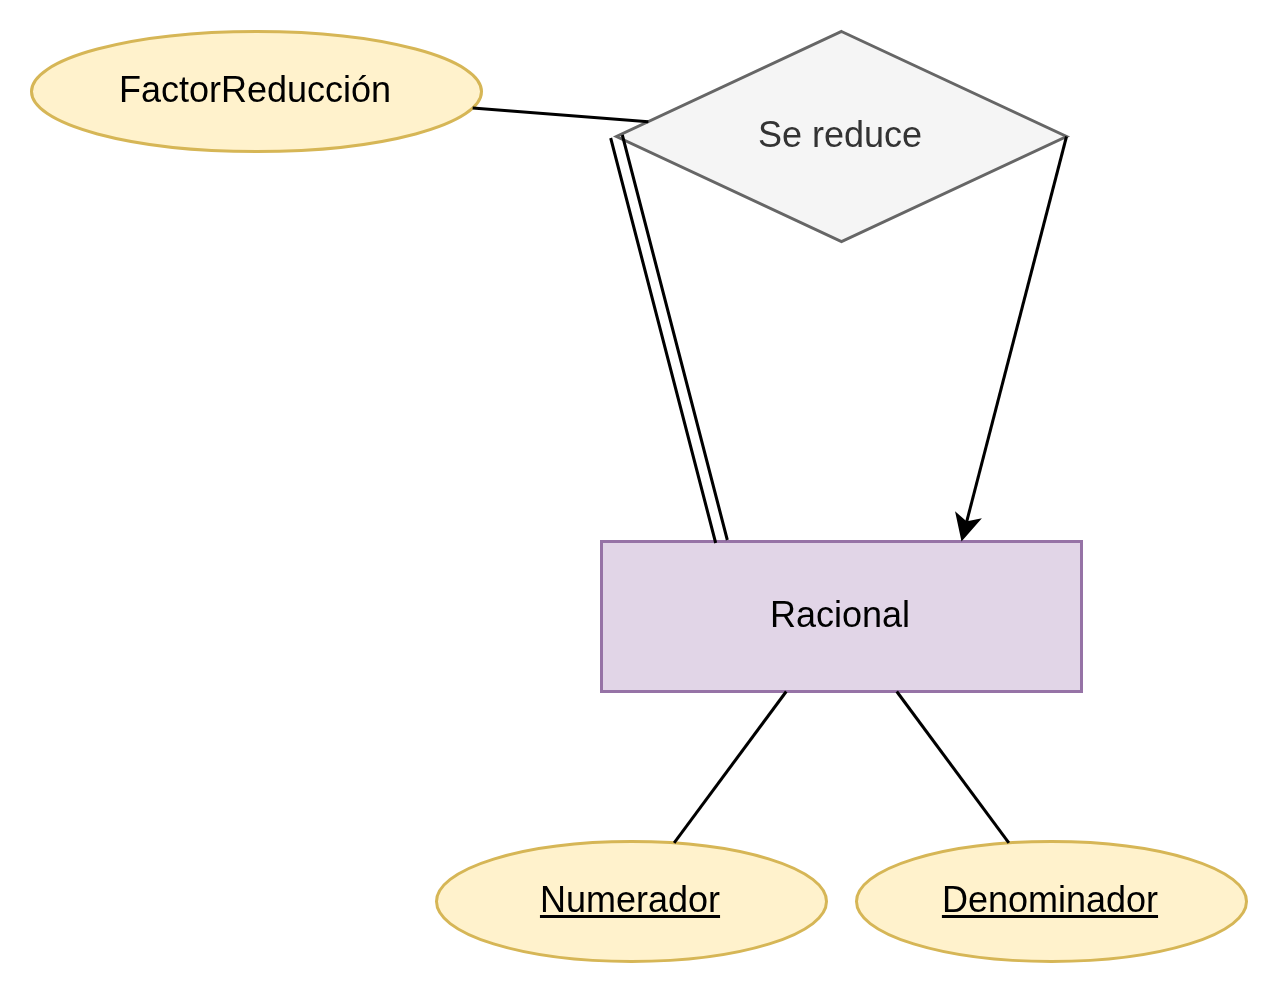
\includegraphics[width=0.8\textwidth]{Figuras/3a_racionales.png}
	\caption{Modelo E-R para números racionales.}
	\label{fig:3a}
\end{figure}

\textbf{Consideraciones de diseño:}

\textbf{1) Identidad de \textit{Racional}.} Un número racional queda determinado por dos enteros, y dos racionales son distintos si difieren en el numerador o en el denominador. Por ello la entidad \textit{Racional} tiene por atributos \textit{Numerador} y \textit{Denominador} y su identificador es la \textbf{clave compuesta (Numerador, Denominador)}.

\textbf{2) Relación recursiva.} El racional reducido de una fracción es, a su vez, un número racional; por eso la asociación se modela como una \textbf{relación recursiva} \textit{Se reduce} sobre \textit{Racional}, con dos roles: \textit{fracción} (el número que se simplifica) y \textit{reducido} (su forma totalmente simplificada).

\textbf{3) Cardinalidad y participación.} Cada fracción tiene \textbf{un único} racional reducido y un reducido es la reducción de \textbf{varias} fracciones, de donde la cardinalidad es \textbf{N:1} (fracción N, reducido 1). La participación del lado \textit{fracción} es \textbf{total} (todo racional tiene su reducido) y la del lado \textit{reducido} es \textbf{parcial}.

\textbf{4) \textit{FactorReducción} como atributo de la relación.} El factor depende del \textbf{par} (fracción, reducido) y no de una sola de las entidades; por eso se modela como \textbf{atributo de \textit{Se reduce}}.
